\documentclass[aspectratio=169, t, 8pt]{beamer}

%------configurando acentos-----------
\usepackage[utf8]{inputenc}
\usepackage[brazil]{babel}

\usepackage{graphicx}

%-------Estilos Beamer---------------
\usetheme{metropolis}
%\usecolortheme{crane}
%\usefonttheme{serif}
\linespread{1.2}

% Personalização de Cores (Exemplo: Minimal Teal)
% Cores Base
\definecolor{BgCanvas}{HTML}{F9F9FB}      % Off-white muito suave
\definecolor{MainText}{HTML}{2B2D42}      % Grafite escuro para alta legibilidade
\definecolor{PrimaryAccent}{HTML}{6B111A} % Az
\definecolor{SunCoastFg}{HTML}{B81D24}
% --- CONFIGURAÇÕES DE TEMA BEAMER ---
%\usetheme{metropolis}

\setbeamertemplate{itemize item}{\textcolor{MainText}{$\bullet$}}
\setbeamertemplate{itemize subitem}{\textcolor{MainText}{\scriptsize$\circ$}}
\setbeamertemplate{itemize 3rditem}{\textcolor{MainText}{\tiny$\blacksquare$}}

\setbeamercolor{background canvas}{bg=BgCanvas}
\setbeamercolor{normal text}{fg=MainText}
\setbeamercolor{frametitle}{bg=SunCoastFg, fg=BgCanvas}
\setbeamercolor{title}{fg=MainText}
\setbeamercolor{subtitle}{fg=PrimaryAccent}
\setbeamercolor{structure}{fg=PrimaryAccent}

% Remove a linha amarela padrão do Metropolis sob o título
\setbeamertemplate{title separator}{}
\setbeamertemplate{progress bar in section page}{}


%--------Dados do Documento
\title{Matemática: Lista de Exercícios}
\author{prof. Eduardo}
\institute{Pré-Universitário Oficina do Saber / UFF}
\date{\today}


%-------- Pacotes Matemática -------------
\usepackage{amsmath}
\usepackage{amsthm}
\usepackage{amsfonts}
\usepackage{amssymb}
\usepackage{xfrac}
\usepackage{thmtools}

%-------- Configuração Listas---------
% \usepackage{enumitem}
\usepackage[inline]{enumitem}

\setcounter{tocdepth}{2}

\newcounter{questaovest}
\newcommand{\vest}{\stepcounter{questaovest}\item[\textbf{Questão \arabic{questaovest}}:]}
\setlist[enumerate]{
    align=left,
    leftmargin=1.8em,
    itemindent=1.8em
    }

\setlist[enumerate,2]{
    label=\alph*.,
    font=\bfseries,
    itemsep=0.1pt,
    labelsep=0em,
    parsep=0pt,
    leftmargin=0em,
    }

%------------- Atalho para imagens ------------
\graphicspath{{../../src/img/semana10/}}


\begin{document}

\begin{frame} %capa
        \vspace*{\fill}
            
            \begin{columns}[c]
                \begin{column}{0.5\textwidth}
                    {\usebeamerfont{title}\usebeamercolor[fg]{title}\inserttitle}\vspace{0.2cm}
                    
                    {\usebeamerfont{subtitle}\usebeamercolor[fg]{subtitle}\insertsubtitle}\vspace{0.5cm}

                {\usebeamerfont{author}\insertauthor}\vspace{0.3cm}

                {\usebeamerfont{institute}\insertinstitute}\vspace{0.3cm}

                {\usebeamerfont{date}\insertdate}
            \end{column}
            
            
            \begin{column}{0.4\textwidth}
                \centering
                
\includegraphics[width=0.4\textwidth]{../logo_ofSaber.png}

                \vspace{.4cm}
                \vspace*{\fill}
        \begin{columns}[c]
            \begin{column}{.5\textwidth}
                \centering
\includegraphics[width=.5\textwidth]{../Proex02c.png}
            \end{column}
            \begin{column}{.5\textwidth}
                \centering
\includegraphics[width=0.4\textwidth]{../Logo_UFF.png}
            \end{column}
        \end{columns}
        \vspace*{\fill}
            \end{column}
        \end{columns}
    \vspace*{\fill}
    \end{frame}
    
        % {
        %     \usebackgroundtemplate{
        %     \includegraphics[width=\paperwidth]{slide_02_contracapa.png}}
        %     \begin{frame}[plain]                
        %     \end{frame}
        % }


    \begin{frame}{Funções}
        \begin{columns}[totalwidth=.9\textwidth]
            \begin{column}{\textwidth}
                \begin{enumerate}
                    \vest{} Considere os conjuntos $A$ (Domínio) e os conjuntos $B$ (Contradomínio). Analise as quatro relações representadas pelos diagramas de flechas abaixo. Com base na definição formal de função, quais das relações apresentadas representam uma função de $A$ em $B$?

                    \vspace{1.2em}

                    \begin{figure}
                        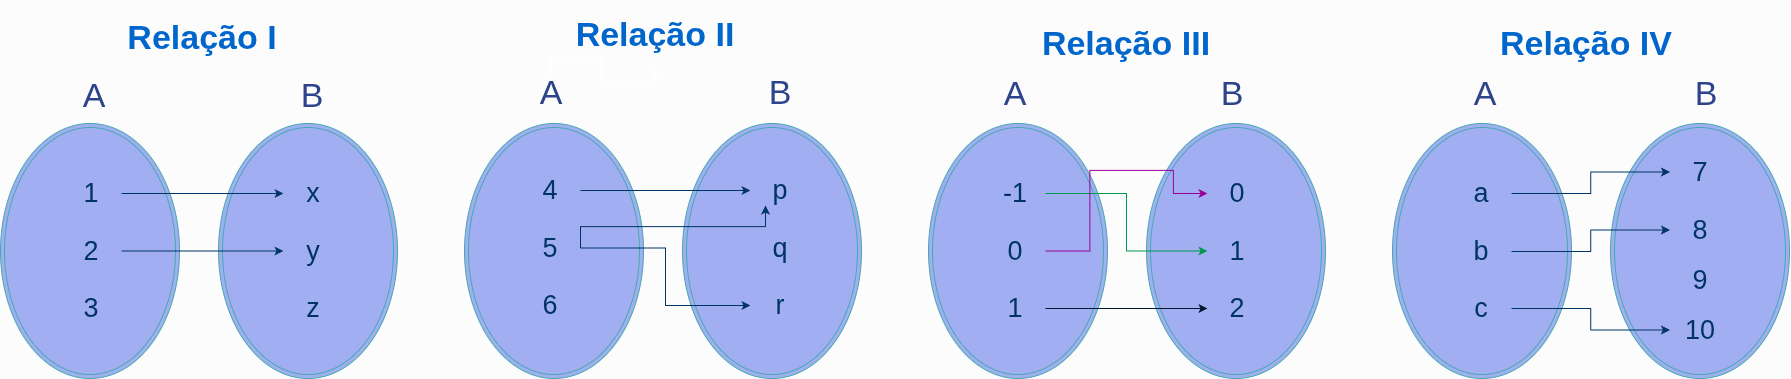
\includegraphics[width=.85\textwidth]{q01_diagrama_funcoes.png}
                    \end{figure}

                    \vspace{2em}

                    \centering
                        \begin{minipage}{.85\textwidth}
                            \begin{enumerate*}[itemjoin={\hfill}]
                                \item \uppercase\expandafter{\romannumeral1 \relax} \text{ e }\uppercase\expandafter{\romannumeral2 \relax}
                                \item \uppercase\expandafter{\romannumeral2 \relax} \text{ e }\uppercase\expandafter{\romannumeral3 \relax}
                                \item \uppercase\expandafter{\romannumeral3 \relax} \text{ e }\uppercase\expandafter{\romannumeral4 \relax}
                                \item \text{Apenas a }\uppercase\expandafter{\romannumeral3 \relax}
                                \item Todas as relações
                                    %gabarito: C
                            \end{enumerate*}
                        \end{minipage}
                \end{enumerate}
            \end{column}
        \end{columns}
    \end{frame}

    \begin{frame}{Funções}
        \begin{columns}[totalwidth=.9\textwidth]
            \begin{column}{\textwidth}
                \begin{enumerate}
                    \vest{Para cada uma das funções abaixo, definidas no conjunto dos números reais ($\mathbb{R}$), determine o domínio de cada uma. Apresente o raciocínio algébrico e a resposta final em notação de conjuntos ou de intervalos.}

                    \vspace{1.2em}

                    \begin{enumerate}
                        \item $\displaystyle f(x) = \frac{7}{x - 5} \vspace{1.1em}$
                        \item $\displaystyle g(x) = \sqrt{2x + 8} \vspace{1.1em}$
                        \item $\displaystyle h(x) = \frac{x}{\sqrt{10 - 2x}} \vspace{1.1em}$
                        \item $\displaystyle p(x) = \frac{\sqrt{x + 3}}{x^2 - 16} \vspace{1.1em}$
                        \item $\displaystyle q(x) = \sqrt{\frac{x - 1}{x - 4}} \vspace{1.1em}$
                    \end{enumerate}
                \end{enumerate}
            \end{column}
        \end{columns}
    \end{frame}

    \begin{frame}{Funções}
        \begin{columns}[totalwidth=.9\textwidth]
            \begin{column}{\textwidth}
                \begin{enumerate}
                    \vest Considere as três funções reais definidas abaixo:

                \vspace{1.2em}
                
                \begin{minipage}{\textwidth}
                    \begin{tabular}{c c c}
                        $f(x) = x^3 - 2x^2 + 5x - 3 \qquad$ & $\displaystyle g(x) = \frac{2x + 4}{x^2 - 1} \qquad$ & $h(x) = \sqrt{3x^2 + 13}$
                    \end{tabular}
                \end{minipage}

                \vspace{1.2em}

                Com base nas leis de formação apresentadas, determine os seguintes valores, apresentando os cálculos passo a passo e simplificando as frações quando necessário:

                \vspace{1em}

                \begin{enumerate}
                    \item $f(-2) \vspace{0.8em}$
                    \item $g(3) \vspace{0.8em}$
                    \item $h(-2) \vspace{0.8em}$
                    \item $f(1)+g(0)-h(2)$
                \end{enumerate}
                \end{enumerate}
            \end{column}
        \end{columns}
    \end{frame}

    \begin{frame}{Funções}
        \begin{columns}[totalwidth=.9\textwidth]
            \begin{column}{\textwidth}
                \begin{enumerate}
                    \vest Em um torneio de xadrez escolar, a comissão organizadora precisa acomodar os competidores no salão principal. Para isso, estabelece-se uma relação matemática $f: J \rightarrow C$, em que $J$ representa o conjunto de jogadores presentes e $C$ representa o conjunto de cadeiras numeradas disponíveis no salão. A regra determina a qual cadeira cada jogador deve se dirigir.
                    
                    \vspace{0.2em}

                    Para que a organização seja perfeita, o professor de matemática exigiu que a função $f$ elaborada pela comissão fosse rigorosamente bijetora.Se a exigência do professor for atendida, qual das situações abaixo deve ser observada no salão?

                    \begin{enumerate}
                        \item O salão possui mais cadeiras do que jogadores, de modo que cada jogador ocupe uma única cadeira e ainda restem lugares vazios.
                        \item O número de jogadores é maior do que o de cadeiras, garantindo que todas as cadeiras sejam ocupadas, embora alguns jogadores tenham que dividir o mesmo assento.
                        \item A quantidade de jogadores é exatamente igual à de cadeiras, sendo que cada jogador ocupa uma cadeira diferente e nenhuma cadeira fica desocupada.
                        \item A quantidade de jogadores e cadeiras é a mesma, mas a regra determina que dois jogadores se sentem juntos em uma mesma cadeira, deixando, consequentemente, uma cadeira vazia.
                        \item Um dos jogadores cadastrados na regra de mapeamento decide não se sentar e fica em pé acompanhando o torneio, enquanto os demais ocupam lugares distintos.
                    \end{enumerate}
                \end{enumerate}
            \end{column}
        \end{columns}
    \end{frame}
    
    \begin{frame}{Funções}
        \begin{columns}[totalwidth=.9\textwidth]
            \begin{column}{\textwidth}
                \begin{enumerate}
                    \vest Considere as funções reais $f(x) = 2x - 3$ e $g(x) = x^2 - x + 4$.

                    Com base nessas leis de formação, resolva os itens a seguir, apresentando todo o desenvolvimento algébrico (passo a passo):

                    \vspace{1.2em}

                    \begin{enumerate}
                        \item Determine a expressão algébrica simplificada da função composta $f(g(x))$. \vspace{3em}
                        \item Determine a expressão algébrica simplificada da função composta $g(f(x))$. \vspace{3em}
                        \item Utilizando as expressões encontradas, calcule o valor numérico de $f(g(2))$ e $g(f(3))$. Com base nos cálculos, determine se a sentença $f(g(2)) \geq g(f(3))$ é verdadeira ou falsa.
                    \end{enumerate}
                \end{enumerate}
            \end{column}
        \end{columns}
    \end{frame}

    \begin{frame}{Funções}
        \begin{columns}[totalwidth=.9\textwidth]
            \begin{column}{\textwidth}
                \begin{enumerate}
                    \vest Um gerente de um cinema observou que, cobrando o valor de R\$ 60,00 pelo ingresso, a média de público em uma sessão normal é de 300 pessoas. Com o objetivo de aumentar o faturamento, ele encomendou uma pesquisa de mercado que revelou o seguinte padrão de comportamento do consumidor: a cada R\$ 1,00 de desconto concedido no preço do ingresso, o público da sessão aumenta em 10 pessoas.

                    \vspace{1em}

                    O gerente decide então reajustar o valor do ingresso para um preço que maximize a receita (faturamento total) arrecadada por sessão.

                    \vspace{1em}

                    Nessas condições, o novo preço do ingresso cobrado pelo cinema deverá ser de:

                    \vspace{.8em}

                    \begin{enumerate}
                        \item $\text{R\$ } 15,00$
                        \item $\text{R\$ } 30,00$
                        \item $\text{R\$ } 45,00$
                        \item $\text{R\$ } 60,00$
                        \item $\text{R\$ } 75,00$
                    \end{enumerate}
                \end{enumerate}
            \end{column}
        \end{columns}
    \end{frame}

    \begin{frame}{Funções}
        \begin{columns}[totalwidth=.9\textwidth]
            \begin{column}{\textwidth}
                \begin{enumerate}
                    \vest  Uma cooperativa agrícola estuda a relação entre a quantidade de um novo fertilizante e a produtividade de suas lavouras de tomate. Pesquisas indicam que a altura média $H$ (em centímetros) atingida pelas plantas após um mês de cultivo depende da quantidade $x$ (em gramas) de fertilizante aplicada semanalmente, sendo modelada pela função $H(x) = -x^2 + 10x + 20$.
                    
                    \vspace{1em}

                    Além disso, os agrônomos descobriram que a produtividade $P$ (em quilogramas de tomate por planta) está diretamente relacionada à altura média $H$ da planta, podendo ser calculada pela função $P(H) = 0,5H + 5$.
                    
                    \vspace{1em}

                    Um agricultor dessa cooperativa decidiu padronizar o seu cultivo, aplicando exatamente 4 gramas semanais do fertilizante em cada planta de sua lavoura.
                    
                    \vspace{1em}
                    
                    Nessas condições, a produtividade esperada por planta, em quilogramas, será de:

                    \vspace{1.2em}
                    
                    \begin{minipage}{.7\textwidth}
                        \begin{enumerate*}[itemjoin={\hfill}]
                            \item 7
                            \item 27
                            \item 43
                            \item 44
                            \item 76 
                        \end{enumerate*}
                    \end{minipage}
                \end{enumerate}
            \end{column}
        \end{columns}
    \end{frame}

\end{document}